\chapter{GPUHElib Design} \label{chap:GPUHElibDesign}
The first attempt at speeding up the run-time of HElib utilizes a GPU to parallelize operations. GPUs are often used to speed up computation where a single instruction or operation is performed on multiple pieces of data. GPUs are ideal for these types of designs because they allow for many compute cores to be run simultaneously, each performing the same operation. HElib utilizes a single instruction, multiple data (SIMD) design, however is single threaded. Meaning that, while being designed so that a single operation occurs over multiple data pieces, the library is not efficiently utilizing the design to best effect. The hope then of adding GPU functionality to the library is to thus take advantage of this design, by utilizing hardware that will best handle the SIMD nature of the scheme. 

There are three phases when executing operations on a GPU. First the memory is copied from the host(CPU) to the device(GPU). Then a kernel is created, which performs the operation on the data in the devices memory. Finally the data is copied back from the device to the host, upon which the host continues execution. These three phases require careful though and implementation in order to achieve the best speedup. 

\section{HElib Serial Design} \label{sec:HElibSerialDesign}

\begin{figure}[htp]
\centering
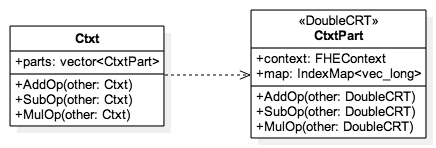
\includegraphics[width=0.65\textwidth]{CtxtTypeHierarchy.png}
\caption{HElib Type Hierarchy}
\label{fig:CtxtTypeHierarchy}
\end{figure}

Let $\ast$ be the operation being perform (here $\ast$ could stand for any of the operations, all of them are handled the similarly) and \textit{A} and \textit{B} be the ciphertexts being operated on. The execution of the operation $A\ \ast\!= B$ requires a few steps. \textit{A} and \textit{B} are stored as \verb|Ctxt| objects in HElib. Figure \ref{fig:CtxtTypeHierarchy} shows the type hierarchy for a \verb|Ctxt| object. \verb|Ctxt| objects have one important variable, \verb|parts|, a vector containing multiple \verb|CtxtPart|s. These parts constitute the ciphertext. The operations supported by \verb|Ctxt| are the addition, subtraction, and multiplication of two \verb|Ctxt| objects. Each of these operations use \verb|parts| during the execution of the operation, thus the operations in \verb|CtxtPart| are called.

\verb|CtxtPart| is an extension of the class \verb|DoubleCRT|, which is where the operations are implemented. Below is code for the operations.

\begin{lstlisting}[language=C++,caption={Add, Sub and Mul operations of two DoubleCRT objects}]
...
const IndexSet& s = map.getIndexSet();
long phim = context.zMStar.getPhiM();

for (long i = s.first(); i <= s.last(); i = s.next(i)) {
    long pi = context.ithPrime(i);
    vec_long& row = map[i];
    const vec_long& other_row = (*other_map)[i];
    
    for (long j = 0; j < phim; j++) {
      row[j] = fun.apply(row[j], other_row[j], pi);
    }
}
...
\end{lstlisting}

As seen in the code above, the index set is iterated over. For each index, the ith prime is extracted along with the ith row from the maps. Even though the map is accessed like an array, it is an unordered map, with the array access syntax for convenience. These rows are then iterated over, applying the operation to each element. This is where the SIMD design is occurring. A double \verb|for| loop to add, subtract or multiply two vectors together. This is where the GPU implementation can occur.

\section{Memory Mapping} \label{sec:MemoryMapping}
In order for the GPU to execute a kernel, it must have the data in a 1D vector. This requires that the data be mapped from its current storage model into a 1D vector.

\subsection{HElib Data Storage and Mapping for GPU Implementation}

\begin{figure}[htp]
\centering
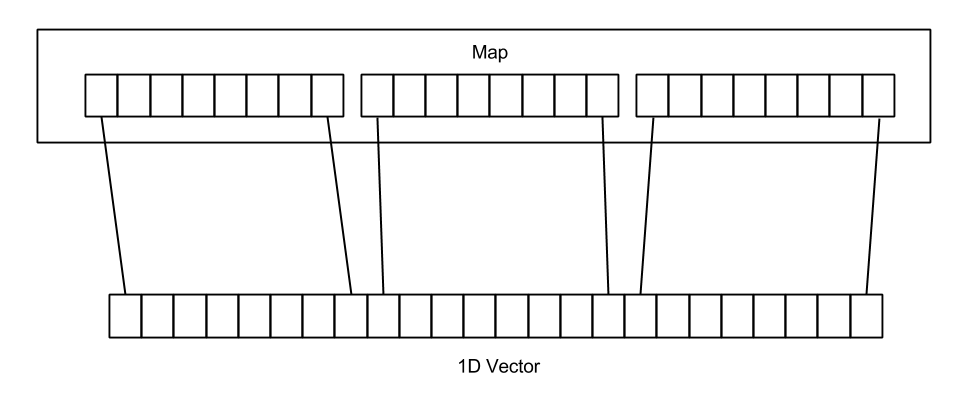
\includegraphics[width=0.65\textwidth]{HElibDataStorage.png}
\caption{HElib Data Storage}
\label{fig:HElibDataStorage}
\end{figure}

Currently the data is stored as shown in Figure \ref{fig:HElibDataStorage}. The \verb|map| contains vectors or rows, each of these rows are arrays of 64-bit integers. This structure is a non-contiguous 1D vector that needs to be mapped to a contiguous 1D vector. Thus the rows must be copied into a new vector, which the GPU will then operate on. Each successive row is concatenated to the preceding rows, thus creating a 1D vector.

\begin{figure}[htp]
\centering
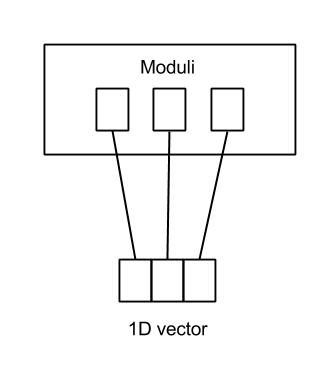
\includegraphics[width=0.3\textwidth]{HElibModuliStorage.png}
\caption{HElib Moduli Storage}
\label{fig:HElibModuliStorage}
\end{figure}

Similarly the moduli are being stored as individual elements. In order to be used during execution on the GPU, they must also be mapped to a 1D vector. Figure \ref{fig:HElibModuliStorage} shows the current storage model for the moduli. Each successive modulus is concatenated to the preceding moduli, thus creating a 1D vector.

\section{Overflow Considerations} \label{sec:OverflowConsiderations}
Six operations were designed, as they are the most commonly used operations. Addition, subtraction, and multiplication of a \verb|DoubleCRT| with another \verb|DoubleCRT| and addition, subtraction, and multiplication of a \verb|DoubleCRT| with a constant number. In CUDA, the language used on NVIDIA GPUs, and the language this implementation is written in, the largest variable type has a length of 64 bits. The type that can contain the largest value is \verb|uint64_t|. This type takes values from 0 to $2^{64} - 1$. 

The type of the data being operated on in HElib is 64-bit signed integers. Meaning they can take values from $-(2^{63})$ to $2^{63} - 1$. However these values will never be negative, thus the actual range of these values is 0 to $2^{63} - 1$. Thus the largest modulus could be the largest possible value, $2^{63} - 1$ and the largest value being operated on could be $2^{63} - 2$. The reason that the largest value being operated on is one less than the largest value, $2^{63} - 1$, is because the value has to be smaller than the modulus, thus $(2^{63} - 1) - 1 = 2^{63} - 2$. The further considerations for overflow prevention will be discussed in the below sections for each operation.

\subsection{Addition Overflow Considerations}
When considering the overflow prevention for addition, it is necessary to compute what the largest value could possibly be. As noted above, the largest a value could be is $2^{63} - 2$ and the largest modulus is $2^{63} - 1$. Performing the addition operation on the possible values, 
\begin{equation} \label{eq:add}
(2^{63} - 2) + (2^{63} - 2) = 2^{64} - 4
\end{equation}
shows that the number $2^{64} - 4$ needs to be computed, before the modulus operation takes place. This number is outside the range for signed 64-bit integers, but not for unsigned 64-bit integers. Thus the original numbers must be cast to unsigned 64-bit integers (which could cause problems if any of the numbers were negative, but since the value are always positive, there is no problem). After the addition operation takes place, the modulus operation brings the result back down the the range of signed integers, because the modulus is in the range of signed integers. The result is then finally cast back to a signed integer, and the operation is complete. The kernels for both addition operations, between two \verb|DoubleCRT| objects and between a \verb|DoubleCRT| object and a constant are in Appendix 
\ref{sec:KernelAddition}.

\subsection{Subtraction Overflow Considerations}
Similar to addition, it is necessary to compute the worst case scenario when considering overflow prevention. Again the largest a value could be is $2^{63} - 2$ and the largest modulus is $2^{63} - 1$. There are two scenarios to consider for subtraction: the first number being $2^{63} - 2$ and the second number being 0 and the first number being 0 and the second number being $2^{63} - 2$. Performing the subtraction operation and modulus calculation for both scenarios
\begin{equation} \label{eq:sub1}
(2^{63} - 2) - 0 = 2^{63} - 2
\end{equation}
\begin{equation} \label{eq:sub2}
0 - (2^{63} - 2) = -(2^{63} - 2)
\end{equation}
shows that all the computations can be completed using signed integers, because all numbers in the above equations are within the range of signed integers. Thus there does not need to be any steps taken to prevent overflow. 

To ensure that the resultant value is greater than 0, a check is then made to determine if the result is less than 0. If so, the modulus is then added to the value, which will result in the value being larger than 0. This check will cause a branch to occur in the GPU, which could slow down run-time. Alternatively, instead of performing a check to determine if the result is less than 0, the modulus can be added to the first value, then the second is subtracted, shown in the below equation, which is a different approach to the subtraction operation. Equation \ref{eq:sub2} is redefined below, with this procedure applied. 
\begin{equation}
(0 + (2^{63} - 1)) - (2^{63} - 2) = (2^{63} - 1) - (2^{63} - 2) = 1
\end{equation}
Now when the modulus operation occurs, the correct result is found, however none of the values throughout the calculation were ever negative. Thus there is no need to perform a check, avoiding the branch, and possible slow down of the run-time. This method however does result in an overflow issue, because the modulus is being added to the first value. Below is this approach applied to Equation \ref{eq:sub1}.
\begin{equation}
((2^{63} - 2) + (2^{63} - 1)) - 0 = (2^{64} - 3) - 0 = (2^{64} - 3)
\end{equation}
This equation generates the value $2^{64} - 3$, which is too large for the signed integer range. Thus a similar procedure to that of addition is performed to ensure overflow prevention. The original numbers are cast to unsigned 64-bit integers. The operation detailed above takes place, before the modulus operation brings the result back down to the signed integer range. The result is then cast back to a signed integer, and completes the operation. The kernels for both subtraction operations, between two \verb|DoubleCRT| objects and between a \verb|DoubleCRT| object and a constant are in Appendix \ref{sec:KernelSubtraction}.

\subsection{Multiplication Overflow Considerations}
Multiplication presents much more problems compared to addition and subtraction. Again the largest value possible is $2^{63} - 2$, with the largest modulus being $2^{63} - 1$. Performing the multiplication operation on these values, 
\begin{equation} \label{eq:mul}
(2^{63} - 2) * (2^{63} - 2) = 2^{126} - 2^{65} + 4
\end{equation}
shows that very large numbers must be generated when performing the multiplication operation. Where for addition and subtraction, the result could fit in a possible data type (unsigned 64-bit integer), these values will not fit in any data type available in CUDA. Therefore an algorithm must be used, which will break up the original numbers into smaller pieces. These pieces will then be used during intermediary steps to generate other values, that when combined back together will result in the correct answer, without ever generating a value that cannot fit in the GPU. The algorithm that is used is Karatsuba's algorithm. 

\subsubsection{Karatsuba's Algorithm}
\begin{equation} \label{eq:Karatsubas}
\begin{split}
x &= x_1 B^m + x_0\\
y &= y_1 B^m + y_0 \cr\\
z_2 &= x_1 y_1\\
z_1 &= x_1 y_0 + x_0 y_1\\
z_0 &= x_0 y_0 \cr\\
xy & = (x_1 B^m + x_0)(y_1 B^m + y_0)\\
 & = z_2 B^{2m} + z_1 B^{m} + z_0
\end{split}
\end{equation}

Equation \ref{eq:Karatsubas} shows Karatsuba's algorithm in general. The values being multiplied are $x$ and $y$. They are broken into pieces $x_1$, $x_0$ and $y_1$, $y_0$ respectively. These pieces are then used to create $z_2$, $z_1$, and $z_0$, which are finally combined with the base number, $B^m$, to generate the original result. For this case $B=2$ and $m=32$. These values will ensure that operations performed throughout the execution of this algorithm never become greater than the maximum 64-bit unsigned integer value. Each of these will be examined more in-depth to see this.

When $x = 2^{63} - 2$, the variables $x_1$ and $x_0$ have values $x_1 = 2^{31} - 1$ and $x_0 = 2^{32} - 2$. The exact same values are assigned to $y_1$ and $y_0$ since $y = x = 2^{63} - 2$. 

Computing $z_2$,
\begin{equation}
\begin{split}
z_2 & = x_1 y_1\\
 & = (2^{31} - 1) (2^{31} - 1)\\
 & = 2^{62} - 2^{32} + 1
\end{split}
\end{equation}
shows that $z_2$ can fit inside a signed 64-bit integers, since the largest possible value is less than $2^{63} - 1$ (the largest value possible for signed 64-bit integers). 

Computing $z_1$,
\begin{equation}
\begin{split}
z_1 & = x_1 y_0 + x_0 y_1\\
 & = 2[(2^{31} - 1) (2^{32} - 2)]\\
 & = 2[2^{63} - 2^{33} + 2]\\
 & = 2^{64} - 2^{34} + 4
\end{split}
\end{equation}
shows that the intermediate pieces can be computed using signed 64-bit integers, however the addition operation causes the result to be in the range of unsigned 64-bit integers. Thus this calculation requires casting the pieces to unsigned 64-bit integers, carrying out the operation to calculate $z_1$, then performing the modulus operation to bring $z_1$ back down to the signed 64-bit integer space.

Computing $z_0$,
\begin{equation}
\begin{split}
z_0 & = x_0 y_0\\
 & = (2^{32} - 2) (2^{32} - 2)\\
 & = 2^{64} - 2^{34} - 4
\end{split}
\end{equation}
shows that $z_0$ must be calculated using unsigned 64-bit integers, since the result is to large for signed 64-bit integers. Thus this calculation also requires casting the pieces to unsigned 64-bit integers, performing the multiplication, before calculating the modulus to bring the result back into the signed 64-bit integer range.

Now that each of the intermediate pieces have been addressed, the final piece needs consideration. Computing $xy$,
\begin{equation}
\begin{split}
xy & = z_2 B^{2m} + z_1 B^{m} + z_0\\
 & = (2^{62} - 2^{32} + 1) (2^{64})\ +\ (2^{63} - 2^{34} + 5) (2^{32})\ +\ (2^{63} - 2^{34} - 3)
\end{split}
\end{equation}
shows that there will be problems computing $z_2 B^{2m}$ and $z_1 B^{m}$. However these can be dealt with deterministically. By performing a loop, multiplying $z_2$ and $z_1$ by 2, 64 and 32 times respectively, performing the modulus operation after every multiplication, one can obtain the correct value, without exceeding the unsigned 64-bit integer limit. Final modulus operations are applied to each addition, finally resulting in the correct value. This value is cast back to a signed 64-bit integer, and the operation is complete. The kernels for both multiplication operations, between two \verb|DoubleCRT| objects and between a \verb|DoubleCRT| object and a constant are in Appendix \ref{sec:KernelMultiplication}.

\section{Concurrency}